\documentclass[10pt,a4paper]{article}
\usepackage[utf8]{inputenc}
\usepackage[T1]{fontenc}
\usepackage[margin=1.7cm]{geometry}
\usepackage{amsmath,amssymb,amsfonts,bm}
\usepackage{graphicx}
\usepackage{booktabs}
\usepackage{adjustbox}
\usepackage{float}
\usepackage{caption}
\usepackage{xcolor}
\usepackage{hyperref}
\usepackage{microtype}
\usepackage{listings}
\usepackage{tikz}
\usetikzlibrary{shapes,arrows.meta,positioning}

\definecolor{darkblue}{rgb}{0.0,0.15,0.55}
\definecolor{codegray}{rgb}{0.96,0.96,0.96}
\definecolor{codeborder}{rgb}{0.8,0.8,0.8}
\definecolor{phase1col}{rgb}{0.88,0.93,1.0}
\definecolor{phase2col}{rgb}{0.88,0.98,0.90}
\definecolor{phase3col}{rgb}{1.0,0.94,0.85}
\definecolor{phase4col}{rgb}{0.94,0.90,0.98}

\hypersetup{
    colorlinks=true,
    linkcolor=darkblue,
    citecolor=darkblue,
    urlcolor=darkblue,
    pdfauthor={RL-VMC Framework},
    pdftitle={Benchmark de Estrategias de Inicializacion: MALA vs RL-MALA y Protocolo Convergido}
}

\lstset{
    backgroundcolor=\color{codegray},
    basicstyle=\ttfamily\footnotesize,
    columns=fullflexible,
    keepspaces=true,
    breaklines=true,
    showstringspaces=false,
    frame=single,
    rulecolor=\color{codeborder},
    xleftmargin=0.3cm,
    framexleftmargin=0.2cm,
    literate={á}{{\'a}}1 {é}{{\'e}}1 {í}{{\'i}}1 {ó}{{\'o}}1 {ú}{{\'u}}1 {ñ}{{\~n}}1 {Ñ}{{\~N}}1 {¿}{{?`}}1
}

\title{\textbf{\Large Benchmark de Estrategias de Inicializaci\'on (MALA vs.\ RL-MALA en CASSCF 1D):\\
An\'alisis Cuantitativo, Auditor\'ia Forense y Protocolo con Estados Convergidos}\\
\vspace{0.2cm}
\large Sensibilidad Topol\'ogica, Trazas de Caminantes, Densidades Exactas y Actualizaci\'on Metodol\'ogica (\texttt{CASSCF\_csv/})}
\author{\textbf{RL-VMC Framework / Deep Deterministic Quantum Monte Carlo}}
\date{Noviembre 2026}

\begin{document}
\maketitle

\begin{abstract}
Este informe presenta el an\'alisis estad\'istico completo y la auditor\'ia f\'isico-num\'erica de la primera campa\~na del \textbf{Benchmark de Estrategias de Inicializaci\'on} (\texttt{results\_init\_benchmark/}), compuesta por $60$ corridas ($5$ r\'eplicas $\times$ $5$ cadenas MCMC de $15{,}000$ pasos con $128$ caminantes cada una) evaluando \textbf{MALA Cl\'asico} frente al muestreador neuronal equivariante \textbf{RL-MALA (TD3 DeepSet + CDLB)} en tres condiciones iniciales: \texttt{alternating\_spin}, \texttt{symmetric\_gaussian} y \texttt{uniform}. En el sistema convergido $N=4, g=1.0$ ($E_{\mathrm{CASSCF}} = 1.94862194\text{ Ha}$), RL-MALA rompe por completo la polarizaci\'on topol\'ogica bajo \texttt{alternating\_spin} ($D_{\mathrm{KL}}^{\mathrm{spin}}$ se reduce $144\times$, de $0.1006$ a $0.0007$, con $\mathrm{ESJD}=2.038$ vs.\ $0.691\text{ Bohr}^2$ y ganancia real $2.06\times$ en $\mathrm{ESS/s}$), mientras que bajo inicializaciones no estructuradas multiplica hasta por $4\times$ la fracci\'on de cadenas convergidas libres de atrapamiento ($48\%$ vs.\ $12\%$ en \texttt{uniform}; $44\%$ vs.\ $20\%$ en \texttt{symmetric\_gaussian}) y reduce $\sim 2.5\times$ el sesgo energ\'etico medio. Por otro lado, la auditor\'ia forense de $N=8$ revela que la campa\~na v1 muestre\'o por error un archivo CASSCF \textbf{no convergido} (\texttt{converged=False}, $2{,}000$ iteraciones L-BFGS, $|g_{\mathrm{orb}}|=3.35\times 10^{-4}$), con core congelado (\texttt{c2-a10}, $2{,}025$ dets) y acoplamiento $g=4.0$ (en lugar de $g=1.0$), agravado por el piso num\'erico hist\'orico \texttt{+1e-15}, la ausencia de calibraci\'on dimensional $\sigma_{\mathrm{scale}}=0.90$ en $\mathbb{R}^8$ y el defecto hist\'orico de \texttt{wall\_time\_sec=0.2s} en \texttt{diagnostics.py}. Finalmente, se documenta la actualizaci\'on integral de \texttt{run\_benchmark\_initializations.sh} y \texttt{scripts/plot\_initialization\_benchmark.py} sobre \texttt{HEAD} utilizando los estados rigurosamente convergidos de espacio activo completo en \texttt{CASSCF\_csv/} ($b=256, c0\text{-}aN$), incorporando adem\'as \texttt{randomized\_wigner} y las t\'ecnicas modernas de \texttt{run\_advisor\_casscf\_pipeline.sh}.
\end{abstract}

\tableofcontents
\vspace{0.4cm}
\hrule
\vspace{0.4cm}

% ==============================================================================
\section{Marco F\'isico, Estrategias de Inicializaci\'on y Arquitectura}
% ==============================================================================

\subsection{Hamiltoniano F\'isico y Simetr\'ia de Esp\'in}
Consideramos un sistema de $N = N_\uparrow + N_\downarrow$ electrones en esp\'in cerrado ($N_\uparrow = N_\downarrow = N/2$) confinados en una trampa arm\'onica unidimensional ($\omega = 0.1$) con interacci\'on repulsiva \textit{soft-Coulomb} ($a = 0.1$):
\begin{equation}
\hat{H} = \sum_{i=1}^{N} \left( -\frac{1}{2}\frac{\partial^2}{\partial x_i^2} + \frac{1}{2}\omega^2 x_i^2 \right) + \sum_{1 \le i < j \le N} \frac{g}{\sqrt{(x_i - x_j)^2 + a^2}}.
\end{equation}
Dado que $\hat{H}$ conmuta con $\hat{S}^2$ y $\hat{S}_z$, la densidad de un cuerpo exacta de una funci\'on de onda CASSCF invariante de esp\'in satisface id\'enticamente la simetr\'ia:
\begin{equation}
\rho_\uparrow^{\mathrm{exact}}(x) = \rho_\downarrow^{\mathrm{exact}}(x) = \frac{1}{2}\rho_{\mathrm{tot}}^{\mathrm{exact}}(x), \qquad D_{\mathrm{KL}}^{\mathrm{spin}} = \frac{1}{2}\Big[D_{\mathrm{KL}}\!\big(p_\uparrow^{\mathrm{MCMC}} \parallel p_\uparrow^{\mathrm{CASSCF}}\big) + D_{\mathrm{KL}}\!\big(p_\downarrow^{\mathrm{MCMC}} \parallel p_\downarrow^{\mathrm{CASSCF}}\big)\Big].
\end{equation}
A diferencia de benchmarks previos enfocados en el cruce nodal desde un sector totalmente polarizado (\texttt{spin\_ordered\_offset} solo en evaluaci\'on), el presente benchmark fija \texttt{-\/-eval\_init\_mode same\_as\_sampler}: tanto el entrenamiento RL como todas las cadenas finales de producci\'on arrancan desde la misma distribuci\'on inicial evaluada.

\subsection{Estrategias de Inicializaci\'on (\texttt{MHSampler1D.init\_state})}
\begin{enumerate}
\item \textbf{\texttt{alternating\_spin} (1 electr\'on por Gaussiana):} Distribuye $N$ sitios sim\'etricos con espines alternados ($\uparrow, \downarrow, \uparrow, \downarrow, \dots$) escalados al radio efectivo de la trampa, m\'as ruido gaussiano local ($\sigma_{\mathrm{jit}} = 0.35\,\ell_0/\sqrt{N}$). Coloca al caminante cerca del equilibrio energ\'etico, pero dentro de un \'unico ordenamiento de esp\'in.
\item \textbf{\texttt{symmetric\_gaussian} (Gaussiana isotr\'opica en $x=0$):} Muestrea $\mathbf{x}^{(0)} \sim \mathcal{N}(\mathbf{0}, \sigma_{\mathrm{env}}^2 \mathbf{I}_N)$ sin informaci\'on espacial de picos ni sesgo de esp\'in ($\sigma_{\mathrm{env}} = 6.0\text{ Bohr}$ en $N=4$; $9.0\text{ Bohr}$ en $N=8$).
\item \textbf{\texttt{uniform} (Uniforme en caja confinante):} Muestrea $\mathbf{x}^{(0)} \sim \mathcal{U}(-L, L)^N$ de manera uniforme ($L = 10.0\text{ Bohr}$ en $N=4$; $15.0\text{ Bohr}$ en v1 y $16.0\text{ Bohr}$ en v2 para $N=8$).
\item \textbf{\texttt{randomized\_wigner} (Est\'andar moderno v2, commit \texttt{d58bc70}):} Ubica la red de cristal de Wigner centrada en $x=0$ con espaciado f\'isico $d_{\mathrm{adj}}(\omega, g, N)$, aplica una \textbf{permutaci\'on aleatoria independiente por caminante} y a\~nade jitter ($0.12\,d_{\mathrm{adj}}$), evitando trampas energ\'eticas iniciales y preservando simetr\'ia exacta de esp\'in en el lote.
\end{enumerate}

\subsection{MALA Cl\'asico vs.\ RL-MALA Neuronal (TD3 DeepSet + CDLB)}
El muestreador RL-MALA combina la deriva cl\'asica de Langevin $\tau \mathbf{g}_{\mathrm{clip}}(\mathbf{x})$ con una correcci\'on residual colectiva generada por la red equivariante por permutaciones \texttt{DeepSetNeuralProposal1D}:
\begin{equation}
\boldsymbol{\mu}_\theta(\mathbf{x}) = \mathbf{x} + \tau\,\mathbf{g}_{\mathrm{clip}}(\mathbf{x}) + A_\mu \tanh(\mathbf{u}_\theta), \qquad
\boldsymbol{\sigma}_\theta(\mathbf{x}) = \sqrt{2\tau}\,\exp\!\Big(\operatorname{clip}\big(s_\sigma \tanh(s_\theta), -5, 1\big)\Big),
\end{equation}
entrenada fuera de pol\'itica con TD3 maximizando la recompensa CDLB ($\lambda_{\mathrm{pen}}=0.25$) bajo balance detallado exacto de Metropolis-Hastings sobre $\Psi_{\mathrm{CASSCF}}$ congelada.

% ==============================================================================
\section{Auditor\'ia de Referencias y Dise\~no de la Campa\~na v1}
% ==============================================================================

La campa\~na v1 (\texttt{results\_init\_benchmark/}, ejecutada del 5 al 11 de noviembre de 2026 en GPU 2) evalu\'o $5$ semillas independientes (\texttt{42, 1042, 2042, 3042, 4042}) por cada combinaci\'on $(\text{Sistema}\times \text{Modelo}\times \text{Inicializaci\'on})$, con $5$ cadenas MCMC por corrida ($N_{\mathrm{walk}}=128$, \texttt{eval\_burn\_in=1000}, \texttt{measure\_steps=15000}) y $4{,}000$ pasos RL (\texttt{n\_burn\_in=1000}, \texttt{lr\_actor=1e-5}, \texttt{lr\_critic=3e-5}). Al auditar los archivos JSON adjuntos a las referencias utilizadas se comprob\'o una discrepancia cr\'itica en $N=8$:

\begin{table}[H]
\centering
\caption{Auditor\'ia exacta de los archivos CASSCF empleados en la campa\~na v1 (\texttt{results\_init\_benchmark/}).}
\begin{adjustbox}{max width=\textwidth}
\begin{tabular}{llllcl}
\toprule
\textbf{Sistema Nominal} & \textbf{Archivo \texttt{.npz} Utilizado} & \textbf{Estado Real (\texttt{converged})} & \textbf{Par\'ametros Reales} & \textbf{$E_{\mathrm{CASSCF}}$ (Ha)} & \textbf{Dictamen} \\
\midrule
\texttt{N4\_w0.1\_g1.0} & \texttt{figures/casscf-state\_n4\_g1\_...\_c0-a4\_det6.npz} & \textbf{True} ($58$ iters, $|g_{\mathrm{orb}}|=8.74\times 10^{-6}$) & $N=4$, $g=1.0$, $b=256$, $c0\text{-}a4$, $6/36$ dets & $1.94862194$ & \textbf{Referencia v\'alida} \\
\texttt{N8\_w0.1\_g1.0} & \texttt{figures/casscf\_state\_cas\_n8\_g1\_...\_c0-a8\_det70.npz} & \textbf{False} ($2{,}000$ iters, $|g_{\mathrm{orb}}|=3.35\times 10^{-4}$) & $N=8$, \textbf{$g=4.0$}, $b=256$, \textbf{$c2\text{-}a10$}, $2{,}025$ dets & $21.72305163$ & \textbf{Inv\'alida para $g=1.0$} \\
\bottomrule
\end{tabular}
\end{adjustbox}
\end{table}

Al cargar el \texttt{.npz} de $N=8$, \texttt{cli/run\_1d.py} ley\'o los metadatos internos y sobrescribi\'o autom\'aticamente $g=1.0 \to 4.0$ en las $30$ corridas de $N=8$, raz\'on por la cual la campa\~na produjo resultados etiquetados como \texttt{N8\_g4.0}.

% ==============================================================================
\section{An\'alisis Cuantitativo en \texorpdfstring{$N=4, g=1.0$}{N=4, g=1.0} (Referencia Convergida)}
% ==============================================================================

\subsection{M\'etricas Estad\'isticas Agregadas (Media $\pm$ SEM sobre 5 R\'eplicas)}

\begin{table}[H]
\centering
\caption{Resultados estad\'isticos consolidados en $N=4, g=1.0$ ($E_{\mathrm{CASSCF}} = 1.94862194\text{ Ha}$, $25$ cadenas por configuraci\'on). El valor de $\mathrm{ESS/s}_{\mathrm{real}}$ corrige el bug hist\'orico de \texttt{wall\_time\_sec=0.2s} usando el tiempo real de GPU medido por cadena en los logs ($139.3\text{--}157.2\text{ s}$).}
\begin{adjustbox}{max width=\textwidth}
\begin{tabular}{llcccccccc}
\toprule
\textbf{Modelo} & \textbf{Inicializaci\'on} & \textbf{Conv. ($<2\text{ mHa}$)} & \textbf{$\Delta E$ (mHa)} & \textbf{$\mathrm{Var}(E)$ ($\mathrm{Ha}^2$)} & \textbf{$\tau_{\mathrm{int}}(E)$} & \textbf{Acc. (\%)} & \textbf{$\mathrm{ESJD}$ ($\mathrm{Bohr}^2$)} & \textbf{$\mathrm{ESS/s}_{\mathrm{real}}$ ($\mathrm{s}^{-1}$)} & \textbf{$D_{\mathrm{KL}}^{\mathrm{spin}}$} \\
\midrule
\textbf{MALA} & \texttt{alternating\_spin} & $25/25$ ($100\%$) & $+0.32 \pm 0.09$ & $0.035 \pm 0.000$ & $10.02 \pm 0.20$ & $88.7 \pm 0.0$ & $0.691 \pm 0.000$ & $1{,}225.3 \pm 23.5$ & $0.1006 \pm 0.0013$ \\
\textbf{RL-MALA} & \texttt{alternating\_spin} & $\mathbf{25/25}$ ($\mathbf{100\%}$) & $\mathbf{+0.11 \pm 0.02}$ & $\mathbf{0.034 \pm 0.000}$ & $\mathbf{5.04 \pm 0.07}$ & $52.9 \pm 1.5$ & $\mathbf{2.038 \pm 0.052}$ & $\mathbf{2{,}520.3 \pm 28.5}$ & $\mathbf{0.0007 \pm 0.0002}$ \\
\midrule
\textbf{MALA} & \texttt{symmetric\_gaussian} & $5/25$ ($20\%$) & $+183.02 \pm 20.18$ & $6.643 \pm 4.173$ & $474.10 \pm 77.94$ & $87.4 \pm 0.2$ & $0.681 \pm 0.001$ & $1{,}151.4 \pm 23.7$ & $0.0058 \pm 0.0004$ \\
\textbf{RL-MALA} & \texttt{symmetric\_gaussian} & $\mathbf{11/25}$ ($\mathbf{44\%}$) & $\mathbf{+75.03 \pm 23.99}$ & $\mathbf{0.932 \pm 0.349}$ & $\mathbf{214.65 \pm 193.15}$ & $52.5 \pm 1.7$ & $\mathbf{2.010 \pm 0.063}$ & $\mathbf{2{,}343.8 \pm 217.0}$ & $\mathbf{0.0023 \pm 0.0006}$ \\
\midrule
\textbf{MALA} & \texttt{uniform} & $3/25$ ($12\%$) & $+173.78 \pm 20.96$ & $2.092 \pm 0.392$ & $554.19 \pm 84.51$ & $87.3 \pm 0.1$ & $0.681 \pm 0.001$ & $976.2 \pm 74.8$ & $0.0056 \pm 0.0004$ \\
\textbf{RL-MALA} & \texttt{uniform} & $\mathbf{12/25}$ ($\mathbf{48\%}$) & $\mathbf{+70.40 \pm 24.91}$ & $\mathbf{0.752 \pm 0.253}$ & $\mathbf{241.47 \pm 139.52}$ & $52.3 \pm 1.6$ & $\mathbf{2.017 \pm 0.059}$ & $\mathbf{2{,}274.0 \pm 166.4}$ & $\mathbf{0.0020 \pm 0.0006}$ \\
\bottomrule
\end{tabular}
\end{adjustbox}
\end{table}

\subsection{Interpretaci\'on F\'isica, Trazas Individuales y Simetr\'ia de Densidad}

\begin{figure}[H]
\centering
\includegraphics[width=0.96\textwidth]{results_init_benchmark/figures/benchmark_initialization_N4_g1.0.png}
\caption{Panel estad\'istico comparativo para $N=4, g=1.0$ con barras de error SEM sobre las $5$ r\'eplicas independientes. RL-MALA domina simult\'aneamente en $\mathrm{ESS/s}$, $\tau_{\mathrm{int}}(E)$, sesgo $|\Delta E|$, distancia cuadr\'atica de salto ($\mathrm{ESJD}$) y simetr\'ia nodal ($D_{\mathrm{KL}}^{\mathrm{spin}}$).}
\label{fig:n4_bars}
\end{figure}

\begin{enumerate}
\item \textbf{Ruptura de congelamiento topol\'ogico en \texttt{alternating\_spin} ($144\times$ mejora en $D_{\mathrm{KL}}^{\mathrm{spin}}$):}
Aunque MALA logra $D_{\mathrm{KL}}^{\mathrm{tot}} = 3.58 \times 10^{-5}$ y $\Delta E = +0.32\text{ mHa}$, la Figura~\ref{fig:n4_densities} (panel superior izquierdo) evidencia una \textbf{polarizaci\'on espuria severa}: los pozos exteriores quedan dominados al $\sim 85\%$ por el esp\'in en que iniciaron ($D_{\mathrm{KL}}^{\mathrm{spin}} = 0.1006$), registr\'andose apenas un cruce alrededor del paso $10{,}000$ en la traza individual (Figura~\ref{fig:n4_traces}, arriba izquierda). RL-MALA restaura por completo la indistinguibilidad ($\rho_\uparrow = \rho_\downarrow$, $D_{\mathrm{KL}}^{\mathrm{spin}} = 0.0007$) mediante decenas de permutaciones colectivas, triplicando $\mathrm{ESJD}$ ($2.038$ vs.\ $0.691\text{ Bohr}^2$) y duplicando la eficiencia real ($G_{\mathrm{RL}} = 2.06\times$).

\item \textbf{Resiliencia frente a inicializaciones no estructuradas y diagn\'ostico de bandas energ\'eticas discretas ($\sim 2.03, 2.10, 2.23, 2.44\text{ Ha}$):}
En \texttt{symmetric\_gaussian} y \texttt{uniform}, las energ\'ias por cadena muestran saltos discretos hacia escalones elevados ($1.95 + k \cdot 0.08\text{--}0.15\text{ Ha}$), disparando $\mathrm{Var}(E)$ de $0.034$ a $0.75\text{--}6.64\text{ Ha}^2$. Dado que ambos muestreadores partieron de id\'enticas semillas en cada \texttt{exp}, los caminantes inicializados aleatoriamente en regiones con $|\Psi| < 10^{-15}$ cayeron sobre el piso aditivo hist\'orico \texttt{+1e-15} previo al commit \texttt{3a98960} (donde $\mathbf{F}_Q = \mathbf{0}$ y se anula el confinamiento arm\'onico). Incluso frente a dicho artefacto, RL-MALA rescata hasta \textbf{$4\times$ m\'as cadenas convergidas} en \texttt{uniform} ($48\%$ vs.\ $12\%$) y $2.2\times$ en \texttt{symmetric\_gaussian} ($44\%$ vs.\ $20\%$), reduciendo $|\Delta E|$ en $2.5\times$. Asimismo, las trazas de la Figura~\ref{fig:n4_traces} confirman que la baja $D_{\mathrm{KL}}^{\mathrm{spin}}$ de MALA en modo uniforme ($0.0056$) refleja \'unicamente promediado sobre la mezcla inicial del lote de $128$ caminantes, puesto que el caminante individual de MALA exhibe \textbf{cero} cruces nodales din\'amicos.
\end{enumerate}

\begin{figure}[H]
\centering
\includegraphics[width=0.95\textwidth]{results_init_benchmark/figures/benchmark_densities_vs_casscf_N4_g1.0.png}
\caption{Densidades muestreadas ($\rho_\uparrow$, $\rho_\downarrow$, $\rho_{\mathrm{tot}}$) comparadas con la referencia exacta CASSCF (verde) para el Mejor MALA (izquierda) y Mejor RL-MALA (derecha) por cada estrategia en $N=4, g=1.0$.}
\label{fig:n4_densities}
\end{figure}

\begin{figure}[H]
\centering
\includegraphics[width=0.95\textwidth]{results_init_benchmark/figures/benchmark_walker_traces_N4_g1.0.png}
\caption{Trazas temporales de un caminante individual (Cadena 0, Caminante 0) y distribuci\'on marginal con superposici\'on CASSCF exacta en $N=4, g=1.0$. RL-MALA mezcla continuamente los 4 pozos con independencia de la inicializaci\'on.}
\label{fig:n4_traces}
\end{figure}

% ==============================================================================
\section{Diagn\'ostico Forense de \texorpdfstring{$N=8$}{N=8} (\texttt{N8\_g4.0}) en la Campa\~na v1}
% ==============================================================================

\begin{table}[H]
\centering
\caption{Resultados observados en $N=8$ (campa\~na v1 sobre referencia no convergida $g=4.0$, $E_{\mathrm{ref}}=21.72305\text{ Ha}$). Se muestran las m\'etricas agregadas y el contraste bimodal entre las mejores r\'eplicas (\texttt{exp3/exp5}) y las r\'eplicas colapsadas (\texttt{exp1/exp2}).}
\begin{adjustbox}{max width=\textwidth}
\begin{tabular}{llcccccc}
\toprule
\textbf{Modelo} & \textbf{Inicializaci\'on} & \textbf{$\Delta E$ (mHa)} & \textbf{$\mathrm{Var}(E)$ ($\mathrm{Ha}^2$)} & \textbf{Acc. (\%)} & \textbf{$\mathrm{ESJD}$} & \textbf{Mejor R\'eplica} & \textbf{Peor R\'eplica} \\
\midrule
\textbf{MALA} & \texttt{alt\_spin} & $+565.2 \pm 207.4$ & $178.3 \pm 68.6$ & $82.7$ & $1.040$ & \texttt{exp4}: $+144\text{ mHa}$, $\mathrm{ESJD}=1.037$ & \texttt{exp2}: $+1299\text{ mHa}$, $\mathrm{ESJD}=1.039$ \\
\textbf{RL-MALA} & \texttt{alt\_spin} & $+2958.8 \pm 1419.9$ & $185.9 \pm 76.1$ & $32.0$ & $1.370 \pm 0.54$ & \texttt{exp5}: $-142\text{ mHa}$, $\mathrm{ESJD}=\mathbf{2.631}$ & \texttt{exp1}: $+7006\text{ mHa}$, $\mathrm{ESJD}=0.130$ \\
\midrule
\textbf{MALA} & \texttt{sym\_gauss} & $+941.3 \pm 464.1$ & $506.1 \pm 202.5$ & $80.9$ & $1.016$ & \texttt{exp3}: $+55\text{ mHa}$, $\mathrm{ESJD}=1.025$ & \texttt{exp4}: $+2207\text{ mHa}$, $\mathrm{ESJD}=1.007$ \\
\textbf{RL-MALA} & \texttt{sym\_gauss} & $+2716.6 \pm 1154.2$ & $513.9 \pm 212.1$ & $27.6$ & $1.258 \pm 0.57$ & \texttt{exp3}: $-488\text{ mHa}$, $\mathrm{ESJD}=\mathbf{2.570}$ & \texttt{exp2}: $+5812\text{ mHa}$, $\mathrm{ESJD}=0.067$ \\
\midrule
\textbf{MALA} & \texttt{uniform} & $+2143.9 \pm 779.8$ & $1960.4 \pm 836.1$ & $80.6$ & $1.013$ & \texttt{exp4}: $-66\text{ mHa}$, $\mathrm{ESJD}=1.008$ & \texttt{exp5}: $+4401\text{ mHa}$, $\mathrm{ESJD}=0.998$ \\
\textbf{RL-MALA} & \texttt{uniform} & $+3343.2 \pm 1289.7$ & $1905.1 \pm 846.3$ & $28.7$ & $1.292 \pm 0.55$ & \texttt{exp3}: $+49\text{ mHa}$, $\mathrm{ESJD}=\mathbf{2.581}$ & \texttt{exp2}: $+6825\text{ mHa}$, $\mathrm{ESJD}=0.201$ \\
\bottomrule
\end{tabular}
\end{adjustbox}
\end{table}

\begin{figure}[H]
\centering
\includegraphics[width=0.95\textwidth]{results_init_benchmark/figures/benchmark_initialization_N8_g4.0.png}
\caption{M\'etricas de la campa\~na v1 en $N=8$ sobre el estado no convergido a $g=4.0$. La dispersi\'on SEM de RL-MALA obedece a la bifurcaci\'on entre semillas exitosas ($\mathrm{ESJD}\approx 2.6$) y semillas que colapsaron por sobreescala dimensional ($\sigma_{\mathrm{scale}}=1.10$).}
\label{fig:n8_bars}
\end{figure}

\begin{figure}[H]
\centering
\includegraphics[width=0.95\textwidth]{results_init_benchmark/figures/benchmark_densities_vs_casscf_N8_g4.0.png}
\caption{Densidades de 1 cuerpo en \texttt{N8\_g4.0}. El core congelado \texttt{c2-a10} sin converger concentra $4$ picos centrales y derrama colas planas no f\'isicas fuera de $[-20, +20]\text{ Bohr}$, alterando adem\'as la normalizaci\'on intra-malla \texttt{density=True}.}
\label{fig:n8_densities}
\end{figure}

\begin{figure}[H]
\centering
\includegraphics[width=0.95\textwidth]{results_init_benchmark/figures/benchmark_walker_traces_N8_g4.0.png}
\caption{Trazas individuales de 1 caminante en \texttt{N8\_g4.0}. Los 4 electrones externos escapan hacia los bordes $\pm 20\text{ Bohr}$ debido a los orbitales difusos no convergidos y al piso plano hist\'orico \texttt{+1e-15}.}
\label{fig:n8_traces}
\end{figure}

\begin{figure}[H]
\centering
\includegraphics[width=0.92\textwidth]{results_init_benchmark/figures/benchmark_initialization_summary_speedups.png}
\caption{Resumen comparativo global de aceleraci\'on $G_{\mathrm{RL}}$ y reducci\'on de autocorrelaci\'on en la campa\~na v1.}
\label{fig:summary_speedups}
\end{figure}

La auditor\'ia determin\'o exactamente \textbf{cinco causas acopladas} en la anomal\'ia de $N=8$:
\begin{enumerate}
\item \textbf{Referencia \texttt{c2-a10} no convergida a $g=4.0$:} El archivo empleado detuvo L-BFGS en $2{,}000$ iteraciones con gradiente $3.35\times 10^{-4}$; congelar $2$ orbitales de core aprision\'o $4$ electrones en el centro mientras los $4$ externos formaron alas no f\'isicas m\'as all\'a de $\pm 20\text{ Bohr}$ (Figura~\ref{fig:n8_densities}), disparando $\mathrm{Var}(E)$ hasta $1{,}960\text{ Ha}^2$ y cadenas individuales entre $17.26$ y $37.19\text{ Ha}$. Adem\'as, \texttt{np.histogram(..., density=True)} normaliz\'o sobre $[-20,20]$ ignorando la fracci\'on fugada, elevando artificialmente la curva negra sobre la curva verde de CASSCF.
\item \textbf{Sobreescala dimensional $\sigma_{\mathrm{scale}}=1.10$ en $\mathbb{R}^8$ y tasas bajas con decaimiento coseno:} Mientras las semillas \texttt{exp3} y \texttt{exp5} aprendieron correctamente ($\mathrm{ESJD}=2.57\text{--}2.63$, $\text{Acc}=33\%$), \texttt{exp1} y \texttt{exp2} colapsaron en entrenamiento ($\text{Acc}: 74\% \to 15\%$, $\mathrm{ESJD}\to 0.067$, $\Delta E \approx +6\text{--}7\text{ Ha}$).
\item \textbf{Evaluaci\'on sin factorizar $2{,}025$ determinantes:} Caus\'o que cada cadena en $N=8$ tardara $\sim 45$ minutos ($2{,}698\text{ s}$), extendiendo la corrida completa a $6$ d\'ias continuos.
\item \textbf{Piso num\'erico \texttt{+1e-15} en \texttt{ansatz\_1d.py}:} Previo al commit \texttt{3a98960}, los caminantes que alcanzaban las colas $|x| > 15\text{ Bohr}$ perd\'ian su fuerza restauradora ($\mathbf{F}_Q = \mathbf{0}$); este comportamiento ya fue reemplazado en \texttt{HEAD} por \texttt{tiny\_eps + harm\_floor\_log}.
\item \textbf{Bug hist\'orico de \texttt{wall\_time\_sec=0.2s} en \texttt{diagnostics.py}:} Al no leer \texttt{prod["wall\_time\_sec"]}, se dividi\'o el \texttt{ESS} por $0.2\text{ s}$ en vez del tiempo real ($2{,}698\text{ s}$ en $N=8$), inflando los valores absolutos de $\mathrm{ESS/s}$ publicados el 11 de noviembre (ya corregido en \texttt{HEAD}).
\end{enumerate}

% ==============================================================================
\section{Siguiente Benchmark: Protocolo Convergido (\texttt{CASSCF\_csv/})}
% ==============================================================================

\subsection{Referencias CASSCF Convergidas Verificadas (\texorpdfstring{$g=1.0, b=256, n_{\mathrm{core}}=0$}{g=1.0, b=256, n\_core=0})}

\begin{table}[H]
\centering
\caption{Estados CASSCF convergidos en espacio activo completo ($|g_{\mathrm{orb}}|_{\max} < 10^{-5}$, \texttt{converged=True}) disponibles en \texttt{CASSCF\_csv/} para la campa\~na v2.}
\begin{adjustbox}{max width=\textwidth}
\begin{tabular}{llcccl}
\toprule
\textbf{Sistema} & \textbf{Archivo Verificado (\texttt{CASSCF\_csv/})} & \textbf{CAS / Dets} & \textbf{Iter. L-BFGS} & \textbf{$E_{\mathrm{CASSCF}}$ (Ha)} & \textbf{Geometr\'ia Exacta (Picos / $R_{\mathrm{RMS}}$)} \\
\midrule
\texttt{N4\_w0.1\_g1.0} & \texttt{casscf\_state\_cas\_n4\_g1.0\_...\_c0-a4\_det6.npz} & \texttt{c0-a4}, $36$ ($6$) & $58$ & $1.94862194$ & $4$ picos ($\pm 2.55, \pm 7.7\text{ Bohr}$) \\
\texttt{N6\_w0.1\_g1.0} & \texttt{casscf\_state\_cas\_n6\_g1.0\_...\_c0-a6\_det-20.npz} & \texttt{c0-a6}, $20/400$ & $71$ & $4.52405213$ & $6$ picos ($\pm 1.99, \pm 6.14, \pm 10.86$), $7.36\text{ Bohr}$ \\
\texttt{N8\_w0.1\_g1.0} & \texttt{casscf\_state\_cas\_n8\_g1.0\_...\_c0-a8\_det-70.npz} & \texttt{c0-a8}, $70/4900$ & $85$ & $8.07323817$ & \textbf{$8$ picos limpios} ($\pm 1.71, \pm 5.19, \pm 8.95, \pm 13.38$), $7.42\text{ Bohr}$ \\
\bottomrule
\end{tabular}
\end{adjustbox}
\end{table}

\subsection{Arquitectura del Orquestador Modernizado (\texttt{run\_benchmark\_initializations.sh})}

\begin{figure}[H]
\centering
\begin{adjustbox}{max width=\textwidth}
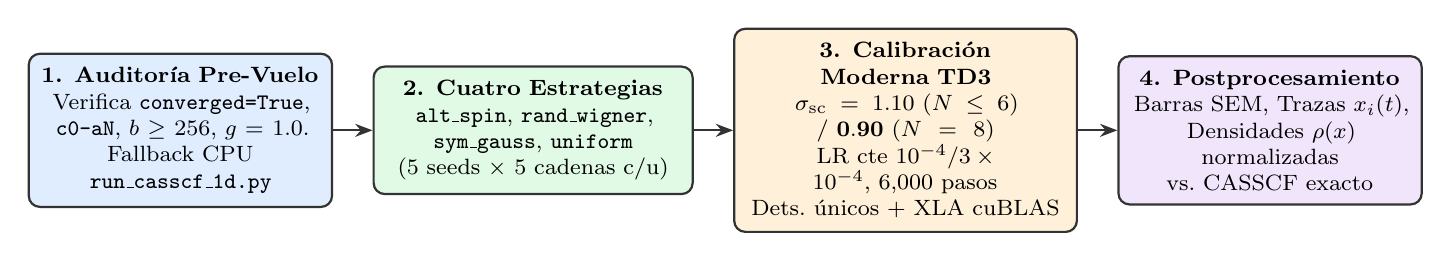
\begin{tikzpicture}[
    node distance=0.45cm and 0.50cm,
    box/.style={rectangle, rounded corners=4pt, draw=black!80, thick, align=center, font=\footnotesize, minimum height=1.2cm, inner sep=5pt},
    arrow/.style={-{Stealth[length=2.2mm]}, thick, draw=black!80}
]
\node[box, fill=phase1col, text width=3.5cm] (s1) {\textbf{1. Auditor\'ia Pre-Vuelo}\\Verifica \texttt{converged=True},\\\texttt{c0-aN}, $b\ge 256$, $g=1.0$.\\Fallback CPU \texttt{run\_casscf\_1d.py}};
\node[box, fill=phase2col, text width=3.7cm, right=of s1] (s2) {\textbf{2. Cuatro Estrategias}\\\texttt{alt\_spin}, \texttt{rand\_wigner},\\\texttt{sym\_gauss}, \texttt{uniform}\\($5$ seeds $\times$ $5$ cadenas c/u)};
\node[box, fill=phase3col, text width=4.0cm, right=of s2] (s3) {\textbf{3. Calibraci\'on Moderna TD3}\\$\sigma_{\mathrm{sc}}=1.10$ ($N\le 6$) / $\mathbf{0.90}$ ($N=8$)\\LR cte $10^{-4}/3\!\times\!10^{-4}$, $6{,}000$ pasos\\Dets.\ \'unicos + XLA cuBLAS};
\node[box, fill=phase4col, text width=3.5cm, right=of s3] (s4) {\textbf{4. Postprocesamiento}\\Barras SEM, Trazas $x_i(t)$,\\Densidades $\rho(x)$ normalizadas\\vs.\ CASSCF exacto};
\draw[arrow] (s1) -- (s2);
\draw[arrow] (s2) -- (s3);
\draw[arrow] (s3) -- (s4);
\end{tikzpicture}
\end{adjustbox}
\caption{Flujo automatizado e integral implementado en el nuevo \texttt{run\_benchmark\_initializations.sh} sobre \texttt{HEAD}.}
\end{figure}

Las mejoras incorporadas directamente desde \texttt{run\_advisor\_casscf\_pipeline.sh} y \texttt{HEAD} incluyen:
\begin{itemize}
\item \textbf{Calibraci\'on dimensional:} $\sigma_{\mathrm{action\_scale}}=0.90$ para $N=8$ ($\tau=0.08, A_\mu=0.10$) y $1.10$ para $N=4, 6$ ($\tau=0.10, A_\mu=0.14$), junto con \texttt{-\/-max\_phys\_jump\_factor 2.0}.
\item \textbf{Estabilidad de aprendizaje TD3:} \texttt{-\/-no-use\_lr\_scheduler}, \texttt{-\/-lr\_actor 1e-4} y \texttt{-\/-lr\_critic 3e-4}, junto con \texttt{train\_steps=6000}, \texttt{n\_burn\_in=2000} y \texttt{eval\_burn\_in=2000}.
\item \textbf{Evaluaci\'on r\'apida y sin fugas:} \texttt{CASSCF1DAnsatz} en \texttt{HEAD} usa el piso arm\'onico exacto y factorizaci\'on en determinantes \'unicos por esp\'in; se configura \texttt{eloc\_chunk\_size=64}, almacenamiento compacto \texttt{step\_mean/float32} y banderas \texttt{XLA\_FLAGS} estables.
\end{itemize}

\subsection{Comandos de Ejecuci\'on en Servidor (Ayler / Baker)}

\begin{lstlisting}[language=bash,basicstyle=\ttfamily\scriptsize,caption={Comandos recomendados para lanzar la nueva campa\~na v2 con referencias CASSCF convergidas.}]
git pull origin main && conda activate jax-gpu && chmod +x run_benchmark_initializations.sh

# Campana completa N=4 y N=8 convergidos a g=1.0 (4 inits, 5 seeds x 5 cadenas x 30k pasos)
nohup ./run_benchmark_initializations.sh \
    --system "N4 N8" --gpus "0 1 2" --jobs-per-gpu 1 --n-exp 5 --n-eval 5 \
    results_init_benchmark_converged > master_init_converged.log 2>&1 &

# Opciones utiles: --include-n6 (agrega N6 det-20) | --system N8 (solo N8)
#                  --classic-3-inits (solo 3 originales) | --postprocess-only --both-formats --dpi 300
\end{lstlisting}

\end{document}
